\documentclass[addpoints,ngerman,12pt,answers]{exam}
\usepackage{babel}
\usepackage[top=2cm,bottom=2.5cm,left=1.5cm,right=1.5cm]{geometry}
\usepackage[utf8]{inputenc}
\usepackage[T1]{fontenc}
\usepackage{booktabs}
\usepackage{graphicx}
\usepackage{csquotes}
\usepackage{paralist}
%\usepackage{wasysym}
%\usepackage[math]{iwona}
\usepackage{setspace}
\usepackage{amsmath} 
\usepackage[math]{iwona}
\usepackage{setspace}
\usepackage{enumitem}
\usepackage{amsmath}
\usepackage{amsfonts}


\pointpoints{Point}{Points}
\bonuspointpoints{Bonuspunkt}{Bonuspunkte}
\renewcommand{\solutiontitle}{\noindent\textbf{Solution:}\enspace}

\chqword{Frage}   
\chpgword{Seite} 
\chpword{Punkte}   
\chbpword{Bonus Points} 
\chsword{Erreicht}   
\chtword{Gesamt}

\checkboxchar{\Square}
\checkedchar{\CheckedBox}

\pagestyle{headandfoot}
\runningheadrule
\firstpageheader{ECO202}{Extra Question F5-F6}{}
\runningheader{ECO202}{Extra Question F5-F6}{}
\firstpagefooter{ECO202}{Extra Question F5-F6}{\thepage\,/\,\numpages}
\runningfooter{ECO202}{Extra Question F5-F6}{\thepage\,/\,\numpages}
\doublespacing

\begin{document}
	\vspace*{3em}
	
	\makebox[\textwidth]{Name:\enspace\hrulefill}
	
	\vspace*{3em}
	\begin{questions}
		
		
		\question In Chapter 4, we delved into the production model. Consider a firm with a production function:
		
		\[Y = AK^{\alpha}L^{1-\alpha}\]
		
		This firm rents capital at a rate of $r$, and the wage rate is $w$.
		
		\begin{enumerate}[label=(\alph*)]
			\item Express the profit maximization problem.
			\item Calculate the Marginal Product of Capital (MPK) and Marginal Product of Labor (MPL). Show the optimal rule to labor and capital hiring.
			\item Determine the appropriate course of action for the firm in the following situations:
			\begin{enumerate}[label=(\roman*)]
				\item When the marginal product of capital exceeds the rental price of capital.
				\item When the marginal product of labor is less than the wage.
			\end{enumerate}
		\end{enumerate}
		
		\clearpage
		\begin{solution}
			\begin{enumerate}[label=(\alph*)]
				\item The firm's objective is to maximize profits, calculated as revenues minus costs:
				
				\(\pi = \text{REV} - \text{COST} = F(K, L) - (rK + wL)\).
				
				The firm determines the quantities of capital, \(K\), and labor, \(L\), to employ, taking into account the prevailing market rental rate for capital, \(r\), and the wage rate, \(w\).
				
				\item The $MPK = \alpha \frac{Y}{K} = \alpha A K^{\alpha - 1} L^{1-\alpha}$ and $MPL= (1-\alpha) \frac{Y}{L}  = (1-\alpha) A K^{\alpha} L^{-\alpha}$
				
				At optimal, the firm would choose $MPK=r$ and $MPL=w$, which
				\[\alpha A K^{\alpha - 1} L^{1-\alpha} = r\]
				\[(1-\alpha) A K^{\alpha} L^{-\alpha} = w\]
				\item 
				\begin{enumerate}[label=(\roman*)]
					\item If MPK is greater than r,  the firm would increase its capital investment since it's producing more output than what it costs to use capital.
					\item if MPL is less than w, the firm should reduce its labor input, as the cost of employing a certain number of laborers exceeds the additional output they contribute to.
				\end{enumerate}
			\end{enumerate}
		\end{solution}		
%		
		\clearpage
		\question This question pertains to the Solow growth model discussed in Chapter 5. Mount Joy, a closed economy without government spending, features a production function:
		
		\[Y_t = A K_t^{1/3} L_t^{2/3}\]
		
		Here, \(Y_t\) represents the output in period \(t\), \(K_t\) denotes the capital in period \(t\), and \(L_t\) stands for the labor employed in period \(t\). Mount Joy's capital accumulation follows the standard function:
		
		\[K_{t+1} = (1 - \delta) K_t + I_t\]
		
		In this equation, \(\delta\) represents the depreciation rate, and \(I_t\) represents the investment in period \(t\).
		
		Mount Joy's population save a proportion \(\bar{s}\) of their output for investment each period. The labor supply is inelastic, with the economy consistently providing \(\bar{L}\) units of labor at any given wage.
		\begin{enumerate}[label=(\alph*)]
			\item Find the steady-state levels of \textit{capital}, \textit{output} and \textit{output per worker} in the Solow model.
			\item If the initial $K_0$ is above its steady state value, show and explain the transition dynamics with clear label for the figure and for the movement.
		\end{enumerate}
		
		\clearpage
		\begin{solution}
			\begin{enumerate}[label=(\alph*)]
				\item We can rewrite the capital accumulation function as 
				\[\Delta K_{t+1} = I_t - \delta K_t = \bar{s}Y - \delta K_t = \bar{s} A  L_t^{2/3} K_t^{1/3} - \delta K_t\]
				In steady state, $\Delta K_{t+1} = 0$
				\[0 = \bar{s} A  L_t^{2/3} K^{1/3} - \delta K\]
				Solving for $K$
				\[K^* =  \left(\frac{\bar{s}}{\delta} A\right)^{3/2}  \bar{L} \]
				Plug it into the production function
				\[Y^* = A \left(\left(\frac{\bar{s}}{\delta} A\right)^{3/2}  \bar{L}\right)^{1/3} \bar{L}^{2/3} = A^{3/2} \left(\frac{\bar{s}}{\delta} \right)^{1/2}  \bar{L} \]
				The steady state output per capita is then
				\[y^* =\frac{Y^*}{L} = A^{3/2} \left(\frac{\bar{s}}{\delta} \right)^{1/2} \]
				\item With $K_0 > K^*$, the the net investment is negative $\bar{s}Y - \delta K_t <0$. This implies the $\Delta K_{t+1} = <0$. With negative net investment, each period, the economy is losing its capital stock and, with less capital available each period, the economy shrinks to the steady state at (K*, Y*) over time
			\end{enumerate}
		\end{solution}
		\begin{figure}[htbp!]
			\centering
			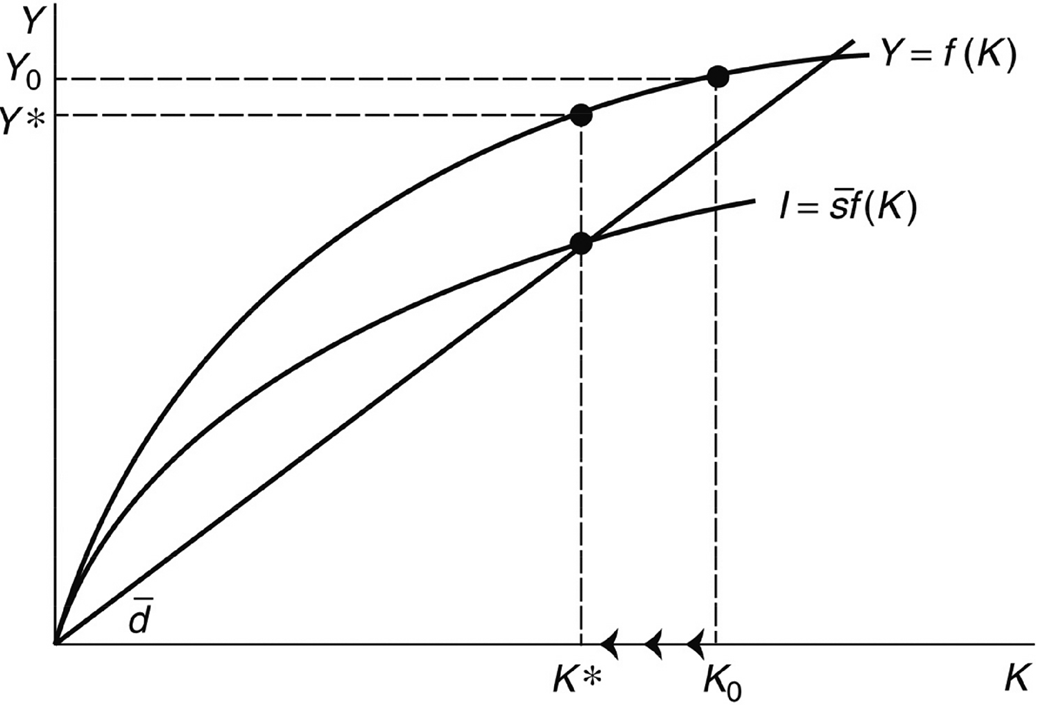
\includegraphics[width=0.7\linewidth]{Figure/screenshot001}
		\end{figure}
	\end{questions}
	
%	\begin{center}
%		\combinedgradetable[h][questions]
%	\end{center}
	
\end{document}